\documentclass[border=8pt]{standalone}
\usepackage[utf8]{inputenc}
\usepackage{tikz}
\usetikzlibrary{positioning}

\tikzset{
  entita/.style = {rectangle, draw, thick, fill=blue!8, minimum width=34mm, minimum height=16mm, font=\small},
  attr/.style   = {circle, draw, thick, fill=white, minimum size=5pt, inner sep=0},
  pk/.style     = {circle, draw, thick, fill=black, minimum size=5pt, inner sep=0},
  link/.style   = {thick},
  et/.style     = {font=\footnotesize}
}

\begin{document}
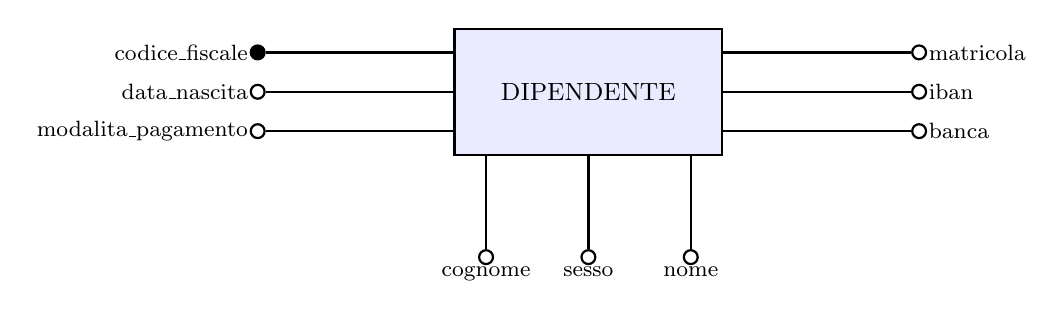
\begin{tikzpicture}

  \node[entita] (E) {DIPENDENTE};

  % lato sinistro
  \node[pk]   (cf)  at (-4.2, 0.5) {}; \draw[link] (-1.7, 0.5) -- (cf);  \node[et,left] at (cf)  {codice\_fiscale};
  \node[attr] (dn)  at (-4.2, 0.0) {}; \draw[link] (-1.7, 0.0) -- (dn);  \node[et,left] at (dn)  {data\_nascita};
  \node[attr] (mp)  at (-4.2,-0.5) {}; \draw[link] (-1.7,-0.5) -- (mp);  \node[et,left] at (mp)  {modalita\_pagamento};

  % lato destro
  \node[attr] (mat) at (4.2, 0.5) {}; \draw[link] (1.7, 0.5) -- (mat); \node[et,right] at (mat) {matricola};
  \node[attr] (ib)  at (4.2, 0.0) {}; \draw[link] (1.7, 0.0) -- (ib);  \node[et,right] at (ib)  {iban};
  \node[attr] (bk)  at (4.2,-0.5) {}; \draw[link] (1.7,-0.5) -- (bk);  \node[et,right] at (bk)  {banca};

  % lato inferiore
  \node[attr] (cog) at (-1.3,-2.1) {}; \draw[link] (-1.3,-0.8) -- (cog); \node[et,below] at (cog) {cognome};
  \node[attr] (ses) at ( 0.0,-2.1) {}; \draw[link] ( 0.0,-0.8) -- (ses); \node[et,below] at (ses) {sesso};
  \node[attr] (nom) at ( 1.3,-2.1) {}; \draw[link] ( 1.3,-0.8) -- (nom); \node[et,below] at (nom) {nome};

\end{tikzpicture}
\end{document}
